\documentclass[conference]{IEEEtran}
\IEEEoverridecommandlockouts

\usepackage{cite}
\usepackage{amsmath,amssymb,amsfonts}
\usepackage{algorithmic}
\usepackage{graphicx}
\usepackage{textcomp}
\usepackage{xcolor}
\usepackage{hyperref}
\def\BibTeX{{\rm B\kern-.05em{\sc i\kern-.025em b}\kern-.08em
    T\kern-.1667em\lower.7ex\hbox{E}\kern-.125emX}}

\begin{document}

    \title{
        MindWatch: Keeping Tech Minds in Balance\\
        {
            \footnotesize \textsuperscript{} \href{https://github.com/Creebos/Mindwatch.git}{https://github.com/Creebos/Mindwatch.git}
        }
    }
    
    \author {
        \IEEEauthorblockN{Riccardo Dennis William}
        \IEEEauthorblockA{\textit{Department of Information System} \\
        \textit{Hanyang University}\\
        Seoul, South Korea \\
        riccaden@students.zhaw.ch}\\
        
        \IEEEauthorblockN{Meyer Yves}
        \IEEEauthorblockA{\textit{Department of Information System} \\
        \textit{Hanyang University}\\
        Seoul, South Korea \\
        meyeryve@students.zhaw.ch} 
        
        \and
    
        \IEEEauthorblockN{Wu Yunjie}
        \IEEEauthorblockA{\textit{Department of Information System} \\
        \textit{Hanyang University}\\
        Seoul, South Korea \\
        19855420423@163.com}\\
    
        \IEEEauthorblockN{Pereira Leandro}
        \IEEEauthorblockA{\textit{Department of Information System} \\
        \textit{Hanyang University}\\
        Seoul, South Korea \\
        pereilea@students.zhaw.ch}
    }
    
    \maketitle
    
    \begin{abstract}
        This project aims to develop a comprehensive web-based
        platform designed to assess the mental health of employees in
        the tech industry through AI-driven analysis of survey
        responses and performance data. The platform will provide
        valuable insights into employee well-being, functioning as an
        early warning system to detect potential mental health concerns
        before they escalate. By offering a dashboard tailored for HR
        professionals, the system enables data-driven decision-making,
        allowing organizations to proactively support employee mental
        health. A key aspect of the platform is the secure handling of
        survey data, ensuring anonymity and confidentiality, which
        fosters trust and encourages widespread adoption among
        employees.
    \end{abstract}
    
    \begin{IEEEkeywords}
        mental health, AI-driven analysis, employee well-being, tech 
        industry, HR dashboard, data security, survey automation, burnout 
        detection, stress management, predictive analytics, human resources,
         data-driven decision-making.
    \end{IEEEkeywords}
    
    
    \begin{table}[htbp]
        \caption{Role Assignments (First half of Project)}
        \centering
        \begin{tabular}{|p{1.8cm}|p{0.9cm}|p{4.8cm}|}
            \hline
            \textbf{Roles} & \textbf{Name} & \textbf{Tasks} \\ \hline
            User & Yunjie & Explaining use-cases and testing demo \\ \hline
            Customer & Leandro & Change use-cases during development \\ \hline
            Software Developer & Leandro, Yunjie, Yves, Dennis & Implementing software and creating model \\ \hline
            Development Manager & Yves, Dennis & Prioritize tasks and organize teams \\ \hline
        \end{tabular}
        \label{tab:role_assignments}
    \end{table}
    
    % refactor?
    \section{Introduction}
    
        The tech industry is known for its high-pressure work environment, 
        often leading to mental health challenges among employees. 
        Early identification of potential mental health risks and timely 
        support can significantly improve employee well-being and overall 
        productivity. However, many organizations lack consistent, 
        confidential tools to monitor and assess mental health across their 
        workforce. This project seeks to address this gap by developing a 
        scalable, AI-powered solution for continuous mental health monitoring.
        
        Tech professionals frequently face long hours, tight
        deadlines, and high-stakes projects, all of which can
        contribute to stress, burnout, and other mental health issues.
        Without proper monitoring tools, organizations risk higher
        turnover rates, decreased productivity, and rising healthcare
        costs. The client, LG, requires a system that will enable HR
        departments to identify early signs of mental health challenges
        before they escalate into more severe problems.\newline
        
        While there are existing platforms such as Headspace and
        Calm, which focus on mental well-being, few solutions offer
        continuous mental health monitoring specifically tailored to
        the tech industry. Furthermore, many available tools lack
        integration with company data or actionable insights for HR
        professionals to drive meaningful interventions. Our platform
        aims to fill this gap by providing continuous, anonymous
        assessments and delivering actionable insights to the HR.
        \newline

    % refactor, add all use cases from diagram
    \section{Requirements}
        
        \subsection{Schedule Survey}
            
            HR managers can schedule periodic mental health surveys
            for employees via the platform. These surveys can be
            customized based on different departments or roles. The
            system ensures that surveys are sent automatically at pre-set
            intervals, allowing organizations to consistently assess
            employee well-being.
            
        \subsection{Fill Out Survey}
                
            Employees will receive and complete mental health
            surveys through the platform. These surveys are designed to
            measure stress, burnout, and other mental health indicators.
            The responses are processed securely to guarantee
            confidentiality, ensuring employees feel comfortable
            providing feedback.
            
        \subsection{Evaluate Mental Health Risk}
                
            The system will analyze survey responses using AI
            algorithms to assess mental health risks. Based on the data
            collected, the system will flag potential issues, such as burnout
            or high stress, and assign a risk level that HR professionals can
            review.
            
        \subsection{Escalate to Psychologist}
                    
            If the system identifies a high mental health risk, or if an
            HR manager requests further investigation, the case can be
            escalated to a psychologist. The psychologist will receive
            relevant reports from the system and can schedule follow-up
            appointments to offer individualized support.
            
        \subsection{Request Report}
                        
             HR managers can generate detailed reports that highlight
             employee mental health trends. These reports provide
             aggregated data and insights into the overall well-being of the
             workforce, helping HR teams identify patterns and implement
             proactive measures.
            
        \subsection{Send Survey Completion Reminder}
        
            If employees fail to complete the survey within a set
            timeframe, the HR managers can send reminders to encourage
            participation. This ensures a higher completion rate and more
            comprehensive data for mental health assessments.
            
        \subsection{Create Incident/Issue}
                       
            Employees and their supervisors can report well-being-
            related incidents or issues directly through the platform. This
            feature allows them to highlight specific concerns or seek
            help, which is then routed to HR or a psychologist based on
            the severity of the issue.
            
        \subsection{Authentication \& Authorization}

            The microservice must enforce secure authentication and authorization protocols, ensuring only authorized users and systems can access its resources. It should support corporate Single Sign-On (SSO) using standards such as OAuth 2.0 and integrate with the organization's Identity Provider (e.g., Azure Active Directory). Role-based access control (RBAC) must be implemented to enforce permissions at a granular level.
        
        \subsection{Scalability}
        
            The microservice should handle variable workloads efficiently by scaling horizontally to add instances during high demand and scaling down during low usage. It must integrate seamlessly with the organization's orchestration tools, such as Kubernetes, to enable automatic scaling while maintaining performance and cost-effectiveness.
            
        \subsection{Maintainability}

            The microservice must be designed with a modular architecture, enabling clear separation of concerns and making it easy to adapt or extend its functionality as requirements evolve. It should facilitate seamless integration with external systems and ensure that connections to third-party services or components can be adjusted or expanded without significant refactoring. The codebase should be clean and structured to minimize the impact of future changes, supporting long-term maintainability and scalability.
    
    \section{Development environment}

        \subsection{Choice of software Development platform}

            Our Application will be split into 4 Components, a Web Frontend, a RESTful API, a database and a AI Model.
            \newline

            \subsubsection{Web Frontend}

                To ensure cross-platform compatibility on Windows, Linux, 
                and macOS, the application's frontend will run in a web 
                browser. It will be built with JavaScript and TypeScript, 
                using the Vue.js framework alongside Bootstrap. 
                \newline
                
                TypeScript is our primary language choice due to its strong typing capabilities, which improve code quality, maintainability, and scalability by reducing errors. This approach supports a smooth experience for employees completing surveys and for HR professionals analyzing data on the dashboard.
                \newline
    
            \subsubsection{RESTful ASP.NET Core API}

                The project’s backend is implemented using ASP.NET Core, 
                a versatile and cross-platform framework ideal for building 
                robust, scalable RESTful APIs. Known for its high performance, ASP.NET Core is compatible with both cloud and container-based deployments, making it an excellent choice for handling the demands of our mental health assessment application. Its modular architecture also allows for efficient maintenance and integration of new features, which is beneficial as the platform evolves. We will be using the newest LTR version, .NET Core 8.0 for our backend application. The most common and essential Libraries we are going to use, should already have released new versions to support 8.0.
                \newline

            \subsubsection{Database}

                For this project, we will be using SQL Server 2022 to manage the database. It’s a straightforward and reliable option for handling structured data with clear relationships, which fits well with the requirements of this project. We will be using Entity Framework Core with a code-first approach to define the database schema directly in C\#, making it easier to manage and adapt as the project evolves. This approach also simplifies database setup and ensures seamless integration between the application and the database. SQL Server’s ease of use and compatibility with .NET make it an ideal choice for a project of this scale.

            \subsubsection{Python (AI Component)}
    
                Python is selected for implementing the AI algorithms for processing survey responses and identifying mental health risks. Its extensive machine learning and natural language processing libraries, such as Scikit-learn, TensorFlow, and NLTK, make Python well-suited for tasks that require sophisticated data analysis. Python’s simplicity and readability are added advantages, enabling the development of complex AI models in a more manageable way, particularly for tasks involving text analysis and sentiment detection within survey responses.
                \newline

            \subsubsection{Docker Containerization}
    
                Our development team operates on multiple operating systems, 
                currently using both Windows and macOS. To streamline our 
                work across platforms and avoid compatibility issues, 
                we decided to use Docker for our entire application, both in 
                development and deployment. Docker enables us to set up on 
                any development machine easily, without requiring installations 
                for .NET, Node, or SQL Server software. 
                \newline
                
                Using Docker is especially beneficial for managing SQL databases, as it simplifies handling ports and local connections that can otherwise be problematic. Additionally, Docker provides us with flexible deployment options for various server environments, allowing us freedom in choosing a server provider. Most modern cloud providers offer native support for Docker, and larger corporations often provide their own managed Kubernetes clusters, allowing us to run our Docker images seamlessly.
                \newline
            
                Our Docker images will be Linux-based for speed and reliability, and there are many prebuilt Docker images available that fit our needs perfectly. We can use ready-made images for SQL Server and use images that run our TypeScript or C-Sharp code with ease.
                \newline

            \subsubsection{Cost estimation}
            
                Since this project is purely for educational purposes, we’ll stick to software that is free for non-commercial use, avoiding the need for licenses. To run our application and support a small number of test users, we won’t require much computing power. There we hope we will be able to find a free platform. Otherwise for cloud hosting, we estimate a budget of around \$5-20 per month.
                \newline

            \subsubsection{Company Environment}
            
                Our application is designed to function as part of a larger corporate ecosystem. While it relies on internal systems typically found in a corporate environment, these systems are not part of our project, as this is a university initiative. To address this, we will create a fictional company environment. To stay within our time constraints, the company will utilize GitHub services, which are quick to set up, easy to use, and free of charge.
    
                For identity management, the company will use GitHub Identity as its Identity Provider. GitHub Repositories will serve as the company's source control system, and we will use repository data as part of our model. The company will also have two internal services:
                
                \begin{itemize}
                    \item An Organization Data Service that provides hierarchical information about the company's employee structure.
                    \item An Attendance Service that tracks employee work hours. The services will expose data through an API, which we will access by pulling the required information.
                \end{itemize}
                
                The company’s infrastructure includes its own Kubernetes cluster for running Docker containers. However, for this project's demonstration, we will use a free platform capable of hosting Docker containers, as the load for this demo will be minimal, and a free-tier solution should suffice.
            

        \subsection {Software in use}

            Since we will be using Docker to build and run our containers, we will install the Docker Desktop app on our development machines.
            \newline

            For the .NET Core backend API, we’ll use Entity Framework with the code-first approach to simplify data storage integration. Additionally, we’ll use OpenAPI Swagger, which provides an API standard and makes it easier to test individual endpoints. For integrating our AI model, we’ll need an additional library, though we haven’t chosen one yet.
            \newline
            
            Our frontend will be built on the Vue.js framework, which includes several built-in libraries. During development, we’ll use Vite to enable real-time updates, allowing our changes to instantly reflect in the running application. Naturally, we’ll also use TypeScript, which is technically external software as well.
            \newline

        \subsection {Task distribution}

            The detailed task distribution for each team member will be 
            developed in the next project phase. This upcoming section 
            will allocate specific responsibilities and roles based 
            on the evolving requirements of the Mental Health Assessment 
            Tool. Each member’s tasks will align closely with the project 
            objectives, focusing on key aspects such as AI model 
            implementation, API development, frontend design, and backend 
            logic. By carefully distributing tasks according to each team 
            member’s expertise, we aim to ensure that all aspects of the 
            project are addressed with clear accountability and focus.
            \newline
    
    \section{Specifications}
    % refactor
    % Technical view and explaination, on how we can achieve the Requirements from II

        \subsection {Functional Requirements}
   
            \begin{itemize}
                \item Schedule Survey 
            \end{itemize}

            The Schedule Survey feature enables HR Managers to organize 
            regular mental health check-ins through scheduled surveys 
            tailored to specific departments or job roles. This feature 
            supports customization in frequency and target audience, 
            allowing surveys to be set up according to the needs of 
            different teams or positions within the organization. 
            \newline

            The backend API in ASP.NET Core provides an endpoint for HR to 
            specify parameters such as survey frequency and targeted 
            departments. The backend also manages survey scheduling 
            logic by storing these configurations in the database, where 
            they are referenced to initiate automatic survey reminders. 
            Through a dedicated dashboard, HR Managers can define and 
            modify survey timing, frequency, and recipients as needed. 
            \newline
        
            All survey schedules are documented in a schedules table 
            within the database, storing parameters like department IDs, 
            job roles, and frequency settings to keep track of survey 
            deployments and for audit purposes.
            \newline
           
            \begin{itemize}
                \item Fill Out Survey 
            \end{itemize}
        
            The Fill Out Survey function allows employees to complete 
            assigned mental health surveys securely and anonymously. 
            Employees receive surveys through the platform and can complete them using a web-based, user-friendly interface. 
            \newline
            
            The frontend form, developed in JavaScript or TypeScript, is designed for ease of use and does not retain any personal information on the client side, prioritizing data privacy. Upon submission, responses are encrypted and processed by the ASP.NET Core backend, ensuring that data is anonymized and securely stored.
            \newline
        
            The backend saves all survey responses in a responses table in 
            the database, which records each entry while maintaining 
            anonymity by linking responses only to anonymized identifiers.
            \newline    
        
            \begin{itemize}
                \item Evaluate Mental Health Risk
            \end{itemize}
            
            The Evaluate Mental Health Risk feature uses AI algorithms to 
            analyze employee responses, assessing their mental health status and assigning risk levels based on survey answers. This automated analysis allows HR to quickly identify trends and potential issues like stress or burnout. The AI component, implemented in Python, applies machine learning models such as logistic regression or decision trees to categorize responses by risk level. Additionally, the platform uses natural language processing (NLP) with libraries like NLTK or SpaCy to preprocess text-based answers, performing sentiment analysis for deeper insight into employee sentiment. \newline
             
            The Python models are accessible via a dedicated API, where the ASP.NET Core backend calls these models after survey completion. Risk assessments are stored in an evaluations table, providing a structured record of mental health evaluations linked to individual survey responses.
            \newline    

            \begin{itemize}
                \item Escalate to Psychologist
            \end{itemize}
    
            For high-risk cases, the Escalate to Psychologist feature 
            provides a pathway for further professional review, allowing 
            HR or the system itself to flag responses for psychologist 
            intervention.
            \newline
    
            The backend includes an API endpoint 
            for escalation requests, which triggers an automatic 
            notification to the psychologist through email or in-app 
            alerts. Details of each escalated case, including the response
            ID, psychologist ID, and relevant timestamps, are stored in an
            escalations table within the database. This feature ensures 
            timely intervention and follow-up on mental health concerns
            flagged by the system.
            \newline    

            \begin{itemize}
                \item Request Report
            \end{itemize}
    
            The Request Report feature provides HR Managers with a 
            comprehensive view of employee mental health trends. The 
            reporting dashboard offers visual summaries through charts, 
            graphs, and other graphical data presentations, providing HR
            with insights into overall well-being within their teams. 
            Developed with tools like Chart.js or D3.js, the dashboard 
            allows HR to explore trends over time and filter data based 
            on department or risk level. \newline
     
            The backend aggregates survey 
            data to produce these insights in real-time, with queries on 
            the responses and evaluations tables to generate trends that 
            are accessible and actionable for HR analysis.
            \newline    

            \begin{itemize}
                \item Send Survey Completion Reminder
            \end{itemize}
    
            The Send Survey Completion Reminder feature improves 
            participation rates by notifying employees who have not 
            completed their surveys within a specified timeframe. The 
            backend includes a scheduled job that periodically checks 
            for incomplete survey entries and automatically sends 
            reminders. \newline
    
            Notifications are dispatched via email or in-app 
            alerts to encourage timely survey completion, helping HR gather 
            accurate, comprehensive data. In the database, completed surveys 
            are flagged in the responses table, while any incomplete entries
            trigger reminders, thus maintaining high response rates and 
            supporting data reliability.
            \newline    

            \begin{itemize}
                \item Create Incident/Issue
            \end{itemize}
    
            The Create Incident/Issue feature enables employees or supervisors 
            to report well-being-related concerns directly on the platform. 
            Through a straightforward form on the frontend, users can report 
            issues, specifying details like incident description, employee ID, 
            and severity level. The backend routes these reports based on their 
            severity to either HR or a psychologist, ensuring each issue is 
            addressed promptly. \newline
            
            Incident details are stored in an incidents
            table in the database, providing a structured record of all 
            reported issues. This system ensures that employee concerns are 
            tracked, documented, and addressed according to severity and 
            relevance
            \newline  
    
        \subsection {Non-Functional Requirements}
   
        \begin{itemize}
            \item Data Security and Privacy
        \end{itemize}
    
        Data Security and Privacy are critical components of the platform, 
        ensuring that all sensitive information is protected throughout the 
        survey process. The platform uses advanced encryption methods like 
        AES or RSA to secure data-at-rest and TLS for data-in-transit, 
        ensuring confidentiality and data protection at all stages. 
        \newline
    
        Role-based access control further secures sensitive information, 
        permitting only authorized personnel, such as HR managers and 
        psychologists, to view or manage confidential data. Compliance with
        standards like GDPR protects employee anonymity, promoting trust 
        and encouraging participation in surveys.
        \newline    

        \begin{itemize}
            \item Scalability
        \end{itemize}
    
        Scalability is achieved through a three-tier architecture, where the 
        frontend, backend, and database layers work independently but in 
        unison. This architecture enables the system to scale efficiently 
        and accommodate growing numbers of users or data loads. 
        \newline
    
        To manage higher concurrent usage, the platform also supports cloud 
        infrastructure options on services like AWS or GCP and can be 
        deployed in Docker containers for modular expansion. These 
        load-balancing and scaling capabilities ensure that the platform 
        remains responsive and effective as the organization expands or as 
        usage increases.
        \newline    

        \begin{itemize}
            \item Accessibility
        \end{itemize}

        The Accessibility of the platform is designed with a responsive, 
        cross-platform interface that supports a range of devices, from 
        Desktops to tablets and mobile phones. The user interface is built 
        to be user-friendly, accommodating employees of all technical 
        backgrounds to maximize engagement and ease of use. By supporting 
        multiple device types and offering a simplified, intuitive user 
        experience, the platform ensures high levels of accessibility, 
        facilitating smooth participation in surveys and effective 
        engagement with the HR dashboard. 
        \newline 

    \section{Architecture Design \& Use Cases}

        \subsection{Overall Architecture}

            \subsubsection{Architecture Design}
            
                The application is designed as a modular system with clear relationships between its components. The main components and their interactions are as follows:
                
                \begin{itemize}
                    \item \textbf{Mindwatch API:} Serves as the central hub, developed with \textit{ASP.NET Core 8} using a RESTful API. It connects to the SQL Server database and coordinates data flow between the frontend, AI Model API, and external services (Organization API and Attendance API).
                    
                    \item \textbf{Mindwatch Frontend:} Built with \textit{Vue.js} and \textit{TypeScript}, the frontend communicates directly with the Mindwatch API to fetch and display employee wellbeing data and AI-driven predictions.
                
                    \item \textbf{AI Model API:} Processes data from surveys and external APIs (Attendance and Organization) to predict stress, burnout risks, and other mental health indicators. It provides predictions back to the Mindwatch API.
                
                    \item \textbf{Database:} A \textit{SQL Server 2022} database stores all survey results, employee data, and prediction outputs. The Mindwatch API uses \textit{Entity Framework Core} (code-first) for data communication.
                
                    \item \textbf{External APIs:} 
                    \begin{itemize}
                        \item \textbf{Organization API:} Supplies organizational hierarchy data for team-based analysis.
                        \item \textbf{Attendance API:} Provides work-hour and attendance data for stress correlation.
                    \end{itemize}
                \end{itemize}
                
                \noindent All components are containerized using \textit{Docker}, with separate containers for the database, API, frontend, and AI model. This architecture ensures seamless communication between services and supports scalability and modularity.
                
                \begin{figure}
                    \centering
                    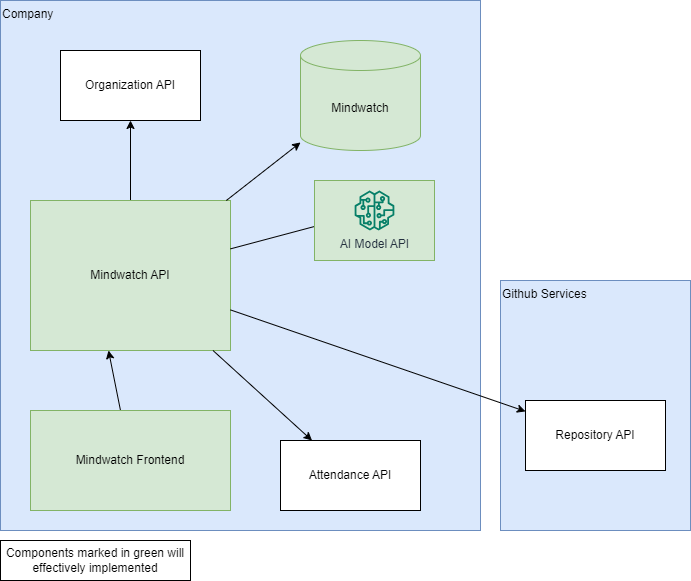
\includegraphics[width=1\linewidth]{DiagramArchitecture.drawio.png}
                    \caption{Architecture of the Mindwatch Application stack}
                    \label{}
                \end{figure}

            \subsubsection{Entity Relationship Diagram}

                The entity-relationship (ER) diagram outlines the database structure and how the entities are connected, forming the foundation for the application. The relationships between the main entities are as follows:
                
                The \textbf{Employee} entity is at the center of the system, representing individual employees. Each employee can belong to one \textbf{Team} (optional) and is linked to various data points, including attendance records, code commits, incidents, and mental health analyses (\textbf{PredictionAnalysis}). These connections allow the system to collect comprehensive information about an employee’s work and wellbeing.
                
                \textbf{Teams} group employees together, enabling team-based analysis of stress or burnout predictions. A team can include multiple employees, but an employee can belong to at most one team.
                
                The \textbf{Questionnaire} entity represents surveys that gather mental health data. Each questionnaire contains multiple \textbf{Questions} and can be assigned to employees through a \textbf{QuestionnaireRun}. A \textbf{QuestionnaireRun} is an instance of a questionnaire being distributed, and it tracks responses submitted by employees. Each run has an associated \textbf{QuestionnaireRunStatus} to indicate its progress or completion.
                
                \textbf{Answers} link employee responses to specific questions in a questionnaire run. An answer is tied to a specific \textbf{Question} and belongs to a particular \textbf{QuestionnaireRun}, ensuring the data remains organized and traceable.
                
                Additional data sources, such as \textbf{Attendance}, \textbf{Commits}, and \textbf{Incidents}, are linked directly to employees:
                - \textbf{Attendance} records track work hours and presence.
                - \textbf{Commits} capture contributions to repositories.
                - \textbf{Incidents} log any work-related events or issues.
                
                Finally, \textbf{PredictionAnalysis} stores the results of AI-driven mental health predictions, directly tied to individual employees. These predictions rely on the aggregated data from questionnaires, attendance, commits, and incidents to provide insights into potential stress or burnout risks.

                \begin{figure}
                    \centering
                    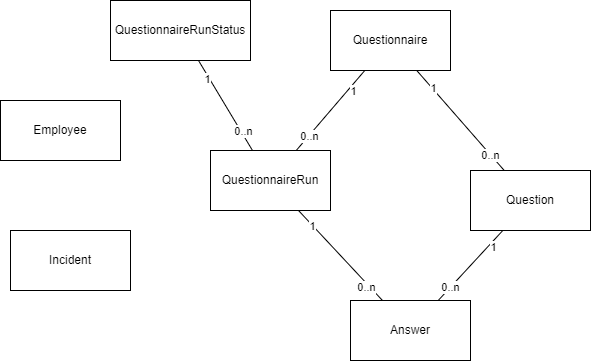
\includegraphics[width=1\linewidth]{DiagramEntityRelationship.drawio.png}
                    \caption{Enter Caption}
                    \label{fig:enter-label}
                \end{figure}


        \subsection{Directory Organization}
            
            \subsection{Project Structure}

                \subsection{Directory Organization}

                    The project structure is divided into general resources, the backend API following the Onion Architecture, and the Vue.js frontend. Below is the detailed breakdown.
                    
                    \subsubsection{General Structure}
                    
   \section{Directory Organization}

        \begin{table}
            \centering
            \renewcommand{\arraystretch}{1.5}
            \begin{tabular}{cc}
                \hline
                \textbf{Directory} & \textbf{Module} \\
                \hline
                \texttt{./docs} & Project Documents\\
                \texttt{./src/AI-Model} & AI Model and Scripts \\
                \texttt{./src/KR.Hanyang.Mindwatch} & Application bundle \\
                \texttt{./src/../..Mindwatch.Api} & Backend API Project \\
                \texttt{./src/../..Mindwatch.Application} & Application Layer \\
                \texttt{./src/../..Mindwatch.Domain} & Domain Layer \\
                \texttt{./src/../..Mindwatch.Frontend} & Frontend Project \\
                \texttt{./src/../..Infrastructure.Persistance} & Persistance Layer \\
                \texttt{./src/Prototype} & Web App Prototype \\
            \end{tabular}
            \caption{Directory and Modules Table}
            \label{tab:my_label}
        \end{table}
                

        \subsection{Project Documents}
            This directory stores all project-related documentation, such as design plans, API specifications, and user manuals. Documentation ensures clear communication within the team and provides reference materials for future maintenance.
        
        \subsection{AI Model and Scripts}
            
            This folder contains the AI models and scripts responsible for processing and predicting employee mental health insights, such as stress or burnout risks. These models are essential for implementing the application's predictive capabilities.
            
        \subsection{Application bundle}
        
            The root directory of the main application bundles all core components together. It contains subdirectories adhering to Onion Architecture principles, with layers for Domain, Application, Infrastructure, and the API.
        \subsection{Backend API Project}

            This module implements the backend API using ASP.NET Core 8. It serves as the entry point for client interactions, exposing RESTful endpoints documented with Swagger (OpenAPI). It communicates with other layers (Application and Domain) to maintain the separation of concerns.
            
        \subsection{Application Layer}
        
            This layer encapsulates business logic, such as handling survey workflows or analyzing mental health data. It defines service contracts and application-specific rules, isolating them from external dependencies.
            
        \subsection{Domain Layer}

            The core of the Onion Architecture, this layer contains business entities and rules. By isolating the domain logic here, the application maintains flexibility and testability, unaffected by changes in infrastructure or presentation.
            
        \subsection{Frontend Project}
                    
            The frontend, developed with Vue.js and TypeScript, provides a user-friendly interface for employees and HR managers. It interacts with the backend API to fetch data and display dashboards, surveys, and AI insights.
            
        \subsection{Persistance Layer}

            This layer handles data access, using Entity Framework Core to manage database operations. It includes migrations, repositories, and database configurations to ensure clean separation from the application logic.
            
        \subsection{Web App Prototype}
        
            A sandbox directory for experimenting with or demonstrating early concepts of the application.

    \section{Use Cases}
        
        \subsection{Use Case 1: Create and Manage Surveys}
        
        \textbf{Description:} HR Managers can create and manage mental health surveys tailored to specific teams or departments. Surveys are distributed periodically to employees, ensuring consistent data collection.
        
        \textbf{Actors:} HR Manager
        
        \textbf{Preconditions:}
        \begin{itemize}
            \item The HR Manager must be authenticated via the company's Identity Platform.
            \item Relevant teams or departments must exist in the system.
        \end{itemize}
        
        \textbf{Flow:}
        \begin{enumerate}
            \item The HR Manager logs into the platform.
            \item The HR Manager navigates to the "Survey Management" dashboard.
            \item A new survey is created by specifying questions, target teams, and scheduling parameters.
            \item The system saves the survey configuration and schedules periodic reminders.
        \end{enumerate}
        
        \textbf{Postconditions:}
        \begin{itemize}
            \item The survey is stored in the database and linked to the specified teams or departments.
            \item The system schedules survey notifications for employees.
        \end{itemize}
        
        \textbf{Exception:}
        \begin{itemize}
            \item If required fields are not provided, the system notifies the HR Manager of the error.
        \end{itemize}
        
        \subsection{Use Case 2: Fill Out Survey}
        
        \textbf{Description:} Employees complete assigned surveys through the platform. Survey responses are securely processed and stored for further analysis.
        
        \textbf{Actors:} Employee
        
        \textbf{Preconditions:}
        \begin{itemize}
            \item The employee must have an active account in the system.
            \item A survey must be assigned to the employee.
        \end{itemize}
        
        \textbf{Flow:}
        \begin{enumerate}
            \item The employee logs into the platform.
            \item The employee views pending surveys on the dashboard.
            \item The employee fills out and submits the survey.
            \item The system validates and encrypts the survey responses before storing them.
        \end{enumerate}
        
        \textbf{Postconditions:}
        \begin{itemize}
            \item The survey response is saved in the database.
            \item The employee's completion status is updated.
        \end{itemize}
        
        \textbf{Exception:}
        \begin{itemize}
            \item If the survey is not submitted before the deadline, the system sends reminders.
        \end{itemize}
        
        \subsection{Use Case 3: Evaluate Mental Health Risks}
        
        \textbf{Description:} The AI Model evaluates survey responses and other data to predict mental health risks such as stress or burnout.
        
        \textbf{Actors:} AI System, HR Manager
        
        \textbf{Preconditions:}
        \begin{itemize}
            \item Survey responses and external data (e.g., attendance, team hierarchy) must be available.
            \item The AI Model must be trained and integrated with the backend.
        \end{itemize}
        
        \textbf{Flow:}
        \begin{enumerate}
            \item The system collects survey responses and additional data.
            \item The AI Model processes the data and calculates risk scores.
            \item The system updates the database with predictions.
            \item The HR Manager views the AI-driven insights on the dashboard.
        \end{enumerate}
        
        \textbf{Postconditions:}
        \begin{itemize}
            \item Risk scores are available for review by HR Managers.
        \end{itemize}
        
        \textbf{Exception:}
        \begin{itemize}
            \item If data is missing or incomplete, the system notifies the relevant parties to address the issue.
        \end{itemize}
        
        \subsection{Use Case 4: Escalate to Psychologist}
        
        \textbf{Description:} High-risk cases are escalated to psychologists for professional intervention.
        
        \textbf{Actors:} HR Manager, Psychologist
        
        \textbf{Preconditions:}
        \begin{itemize}
            \item A high-risk case must be identified by the AI Model or flagged by an HR Manager.
            \item Psychologist accounts must exist in the system.
        \end{itemize}
        
        \textbf{Flow:}
        \begin{enumerate}
            \item The HR Manager flags a high-risk case for escalation.
            \item The system generates a detailed report and sends a notification to the assigned psychologist.
            \item The psychologist reviews the case and schedules follow-up actions.
        \end{enumerate}
        
        \textbf{Postconditions:}
        \begin{itemize}
            \item The high-risk case is tracked in the system for resolution.
        \end{itemize}
        
        \textbf{Exception:}
        \begin{itemize}
            \item If no psychologist is assigned, the system alerts the HR Manager to assign one.
        \end{itemize}
        
        \subsection{Use Case 5: Generate Reports}
        
        \textbf{Description:} HR Managers can request and view detailed reports of employee mental health trends and predictions.
        
        \textbf{Actors:} HR Manager
        
        \textbf{Preconditions:}
        \begin{itemize}
            \item The HR Manager must be authenticated and authorized.
        \end{itemize}
        
        \textbf{Flow:}
        \begin{enumerate}
            \item The HR Manager navigates to the "Reports" section of the dashboard.
            \item A report is requested based on parameters such as department, date range, or risk level.
            \item The system queries the database and generates the report.
            \item The HR Manager views or downloads the report.
        \end{enumerate}
        
        \textbf{Postconditions:}
        \begin{itemize}
            \item The report is available for review, providing actionable insights.
        \end{itemize}
        
        \textbf{Exception:}
        \begin{itemize}
            \item If no data matches the selected parameters, the system notifies the HR Manager.
        \end{itemize}
        

    

\end{document}